\section{Question 2}
System:
$$
G_{1_{(s)}} = \dfrac{1}{(17s+1)(5s+1)}\exp(-30s) = \dfrac{1}{102s^2+23s+1}
$$
We use Optimal PID to design controller with ITAE, ISE and IAE cost function. In program we use 100 second for optimization but use 1000 second for simulation beacuse optimization takes too long time and in 100 second beacuse of long delay time we can't see system behavior. 
\newpage
 \begin{itemize}
     \item ITAE
     $$
     K_p = 0.6867, \quad K_i = 0.0347, \quad K_d = 15.0543
     $$
     \begin{figure}[H]
        \caption{Step responde with PID controller and ITAE cost function}
        \centering
        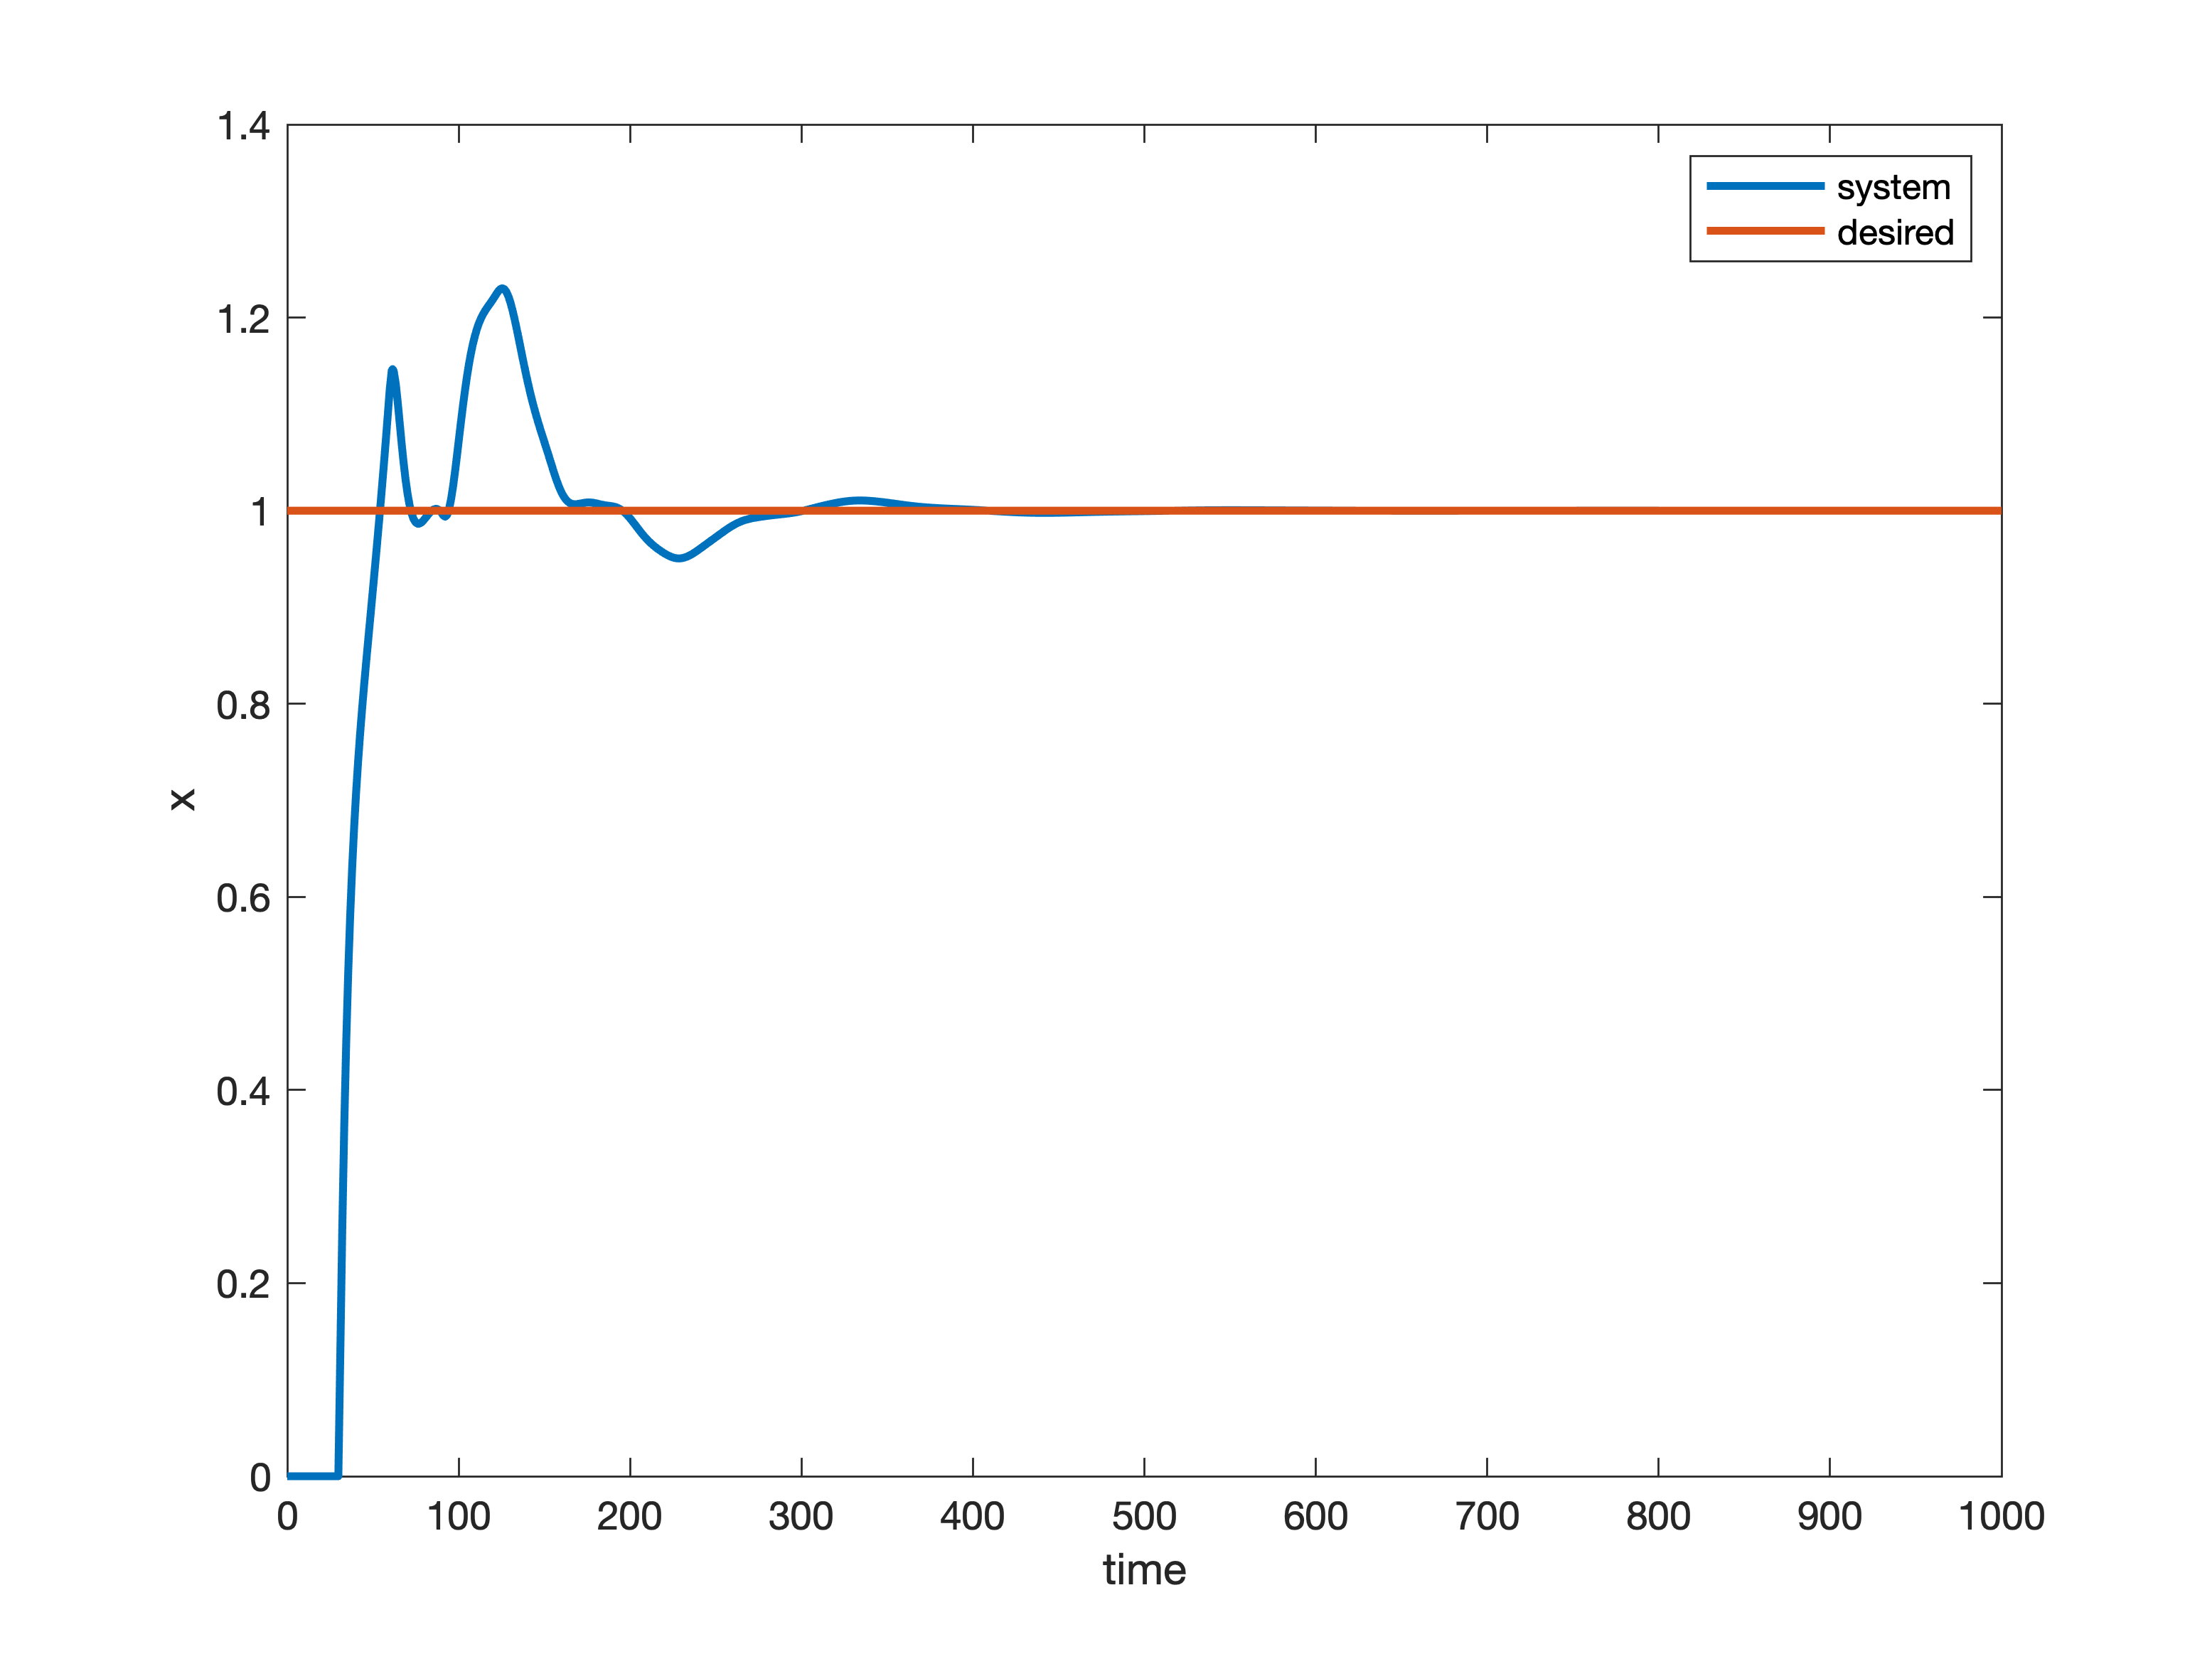
\includegraphics[width=11cm]{../Figure/Q2/ITAE.png}
    \end{figure}
    \item ISE
    $$
    K_p =0.5399, \quad K_i = 0.0446, \quad  K_d =20.8391
    $$
    \begin{figure}[H]
       \caption{Step responde with PID controller and ISE cost function}
       \centering
       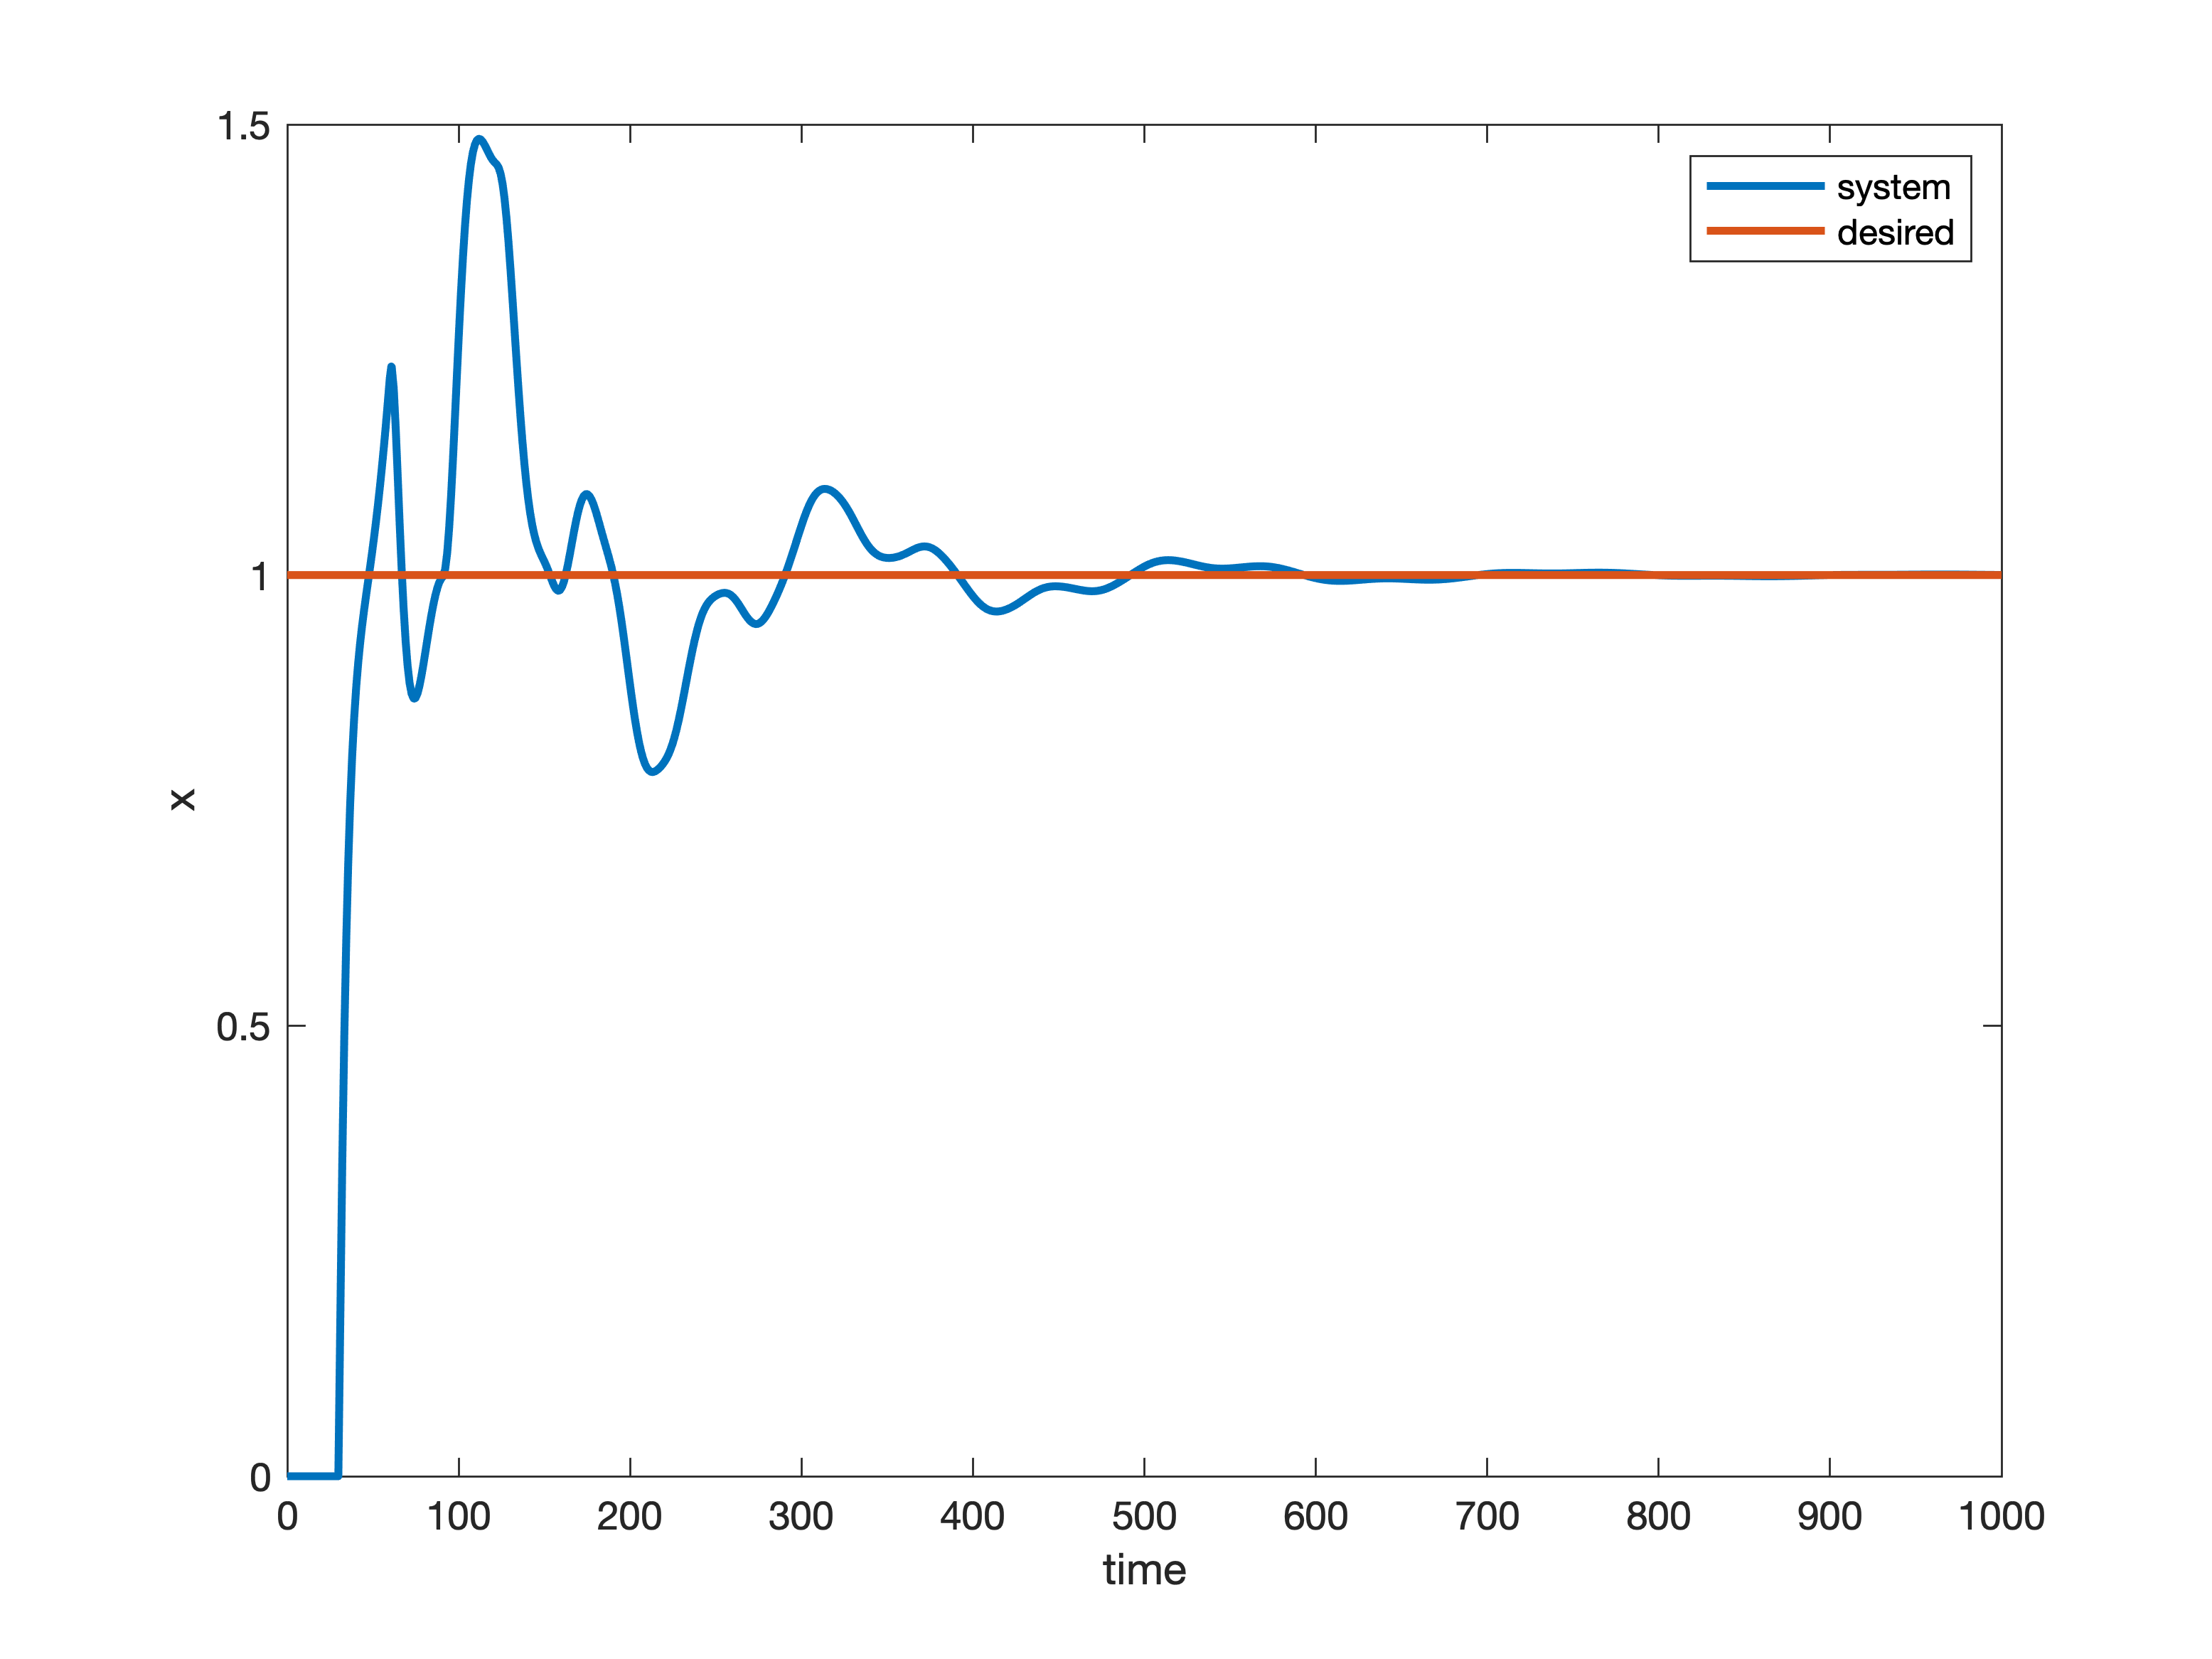
\includegraphics[width=11cm]{../Figure/Q2/ISE.png}
   \end{figure}
   \item IAE
   $$
   K_p = 0.6522, \quad K_i = 0.0393, \quad K_d = 17.5028
   $$
   \begin{figure}[H]
      \caption{Step responde with PID controller and IAE cost function}
      \centering
      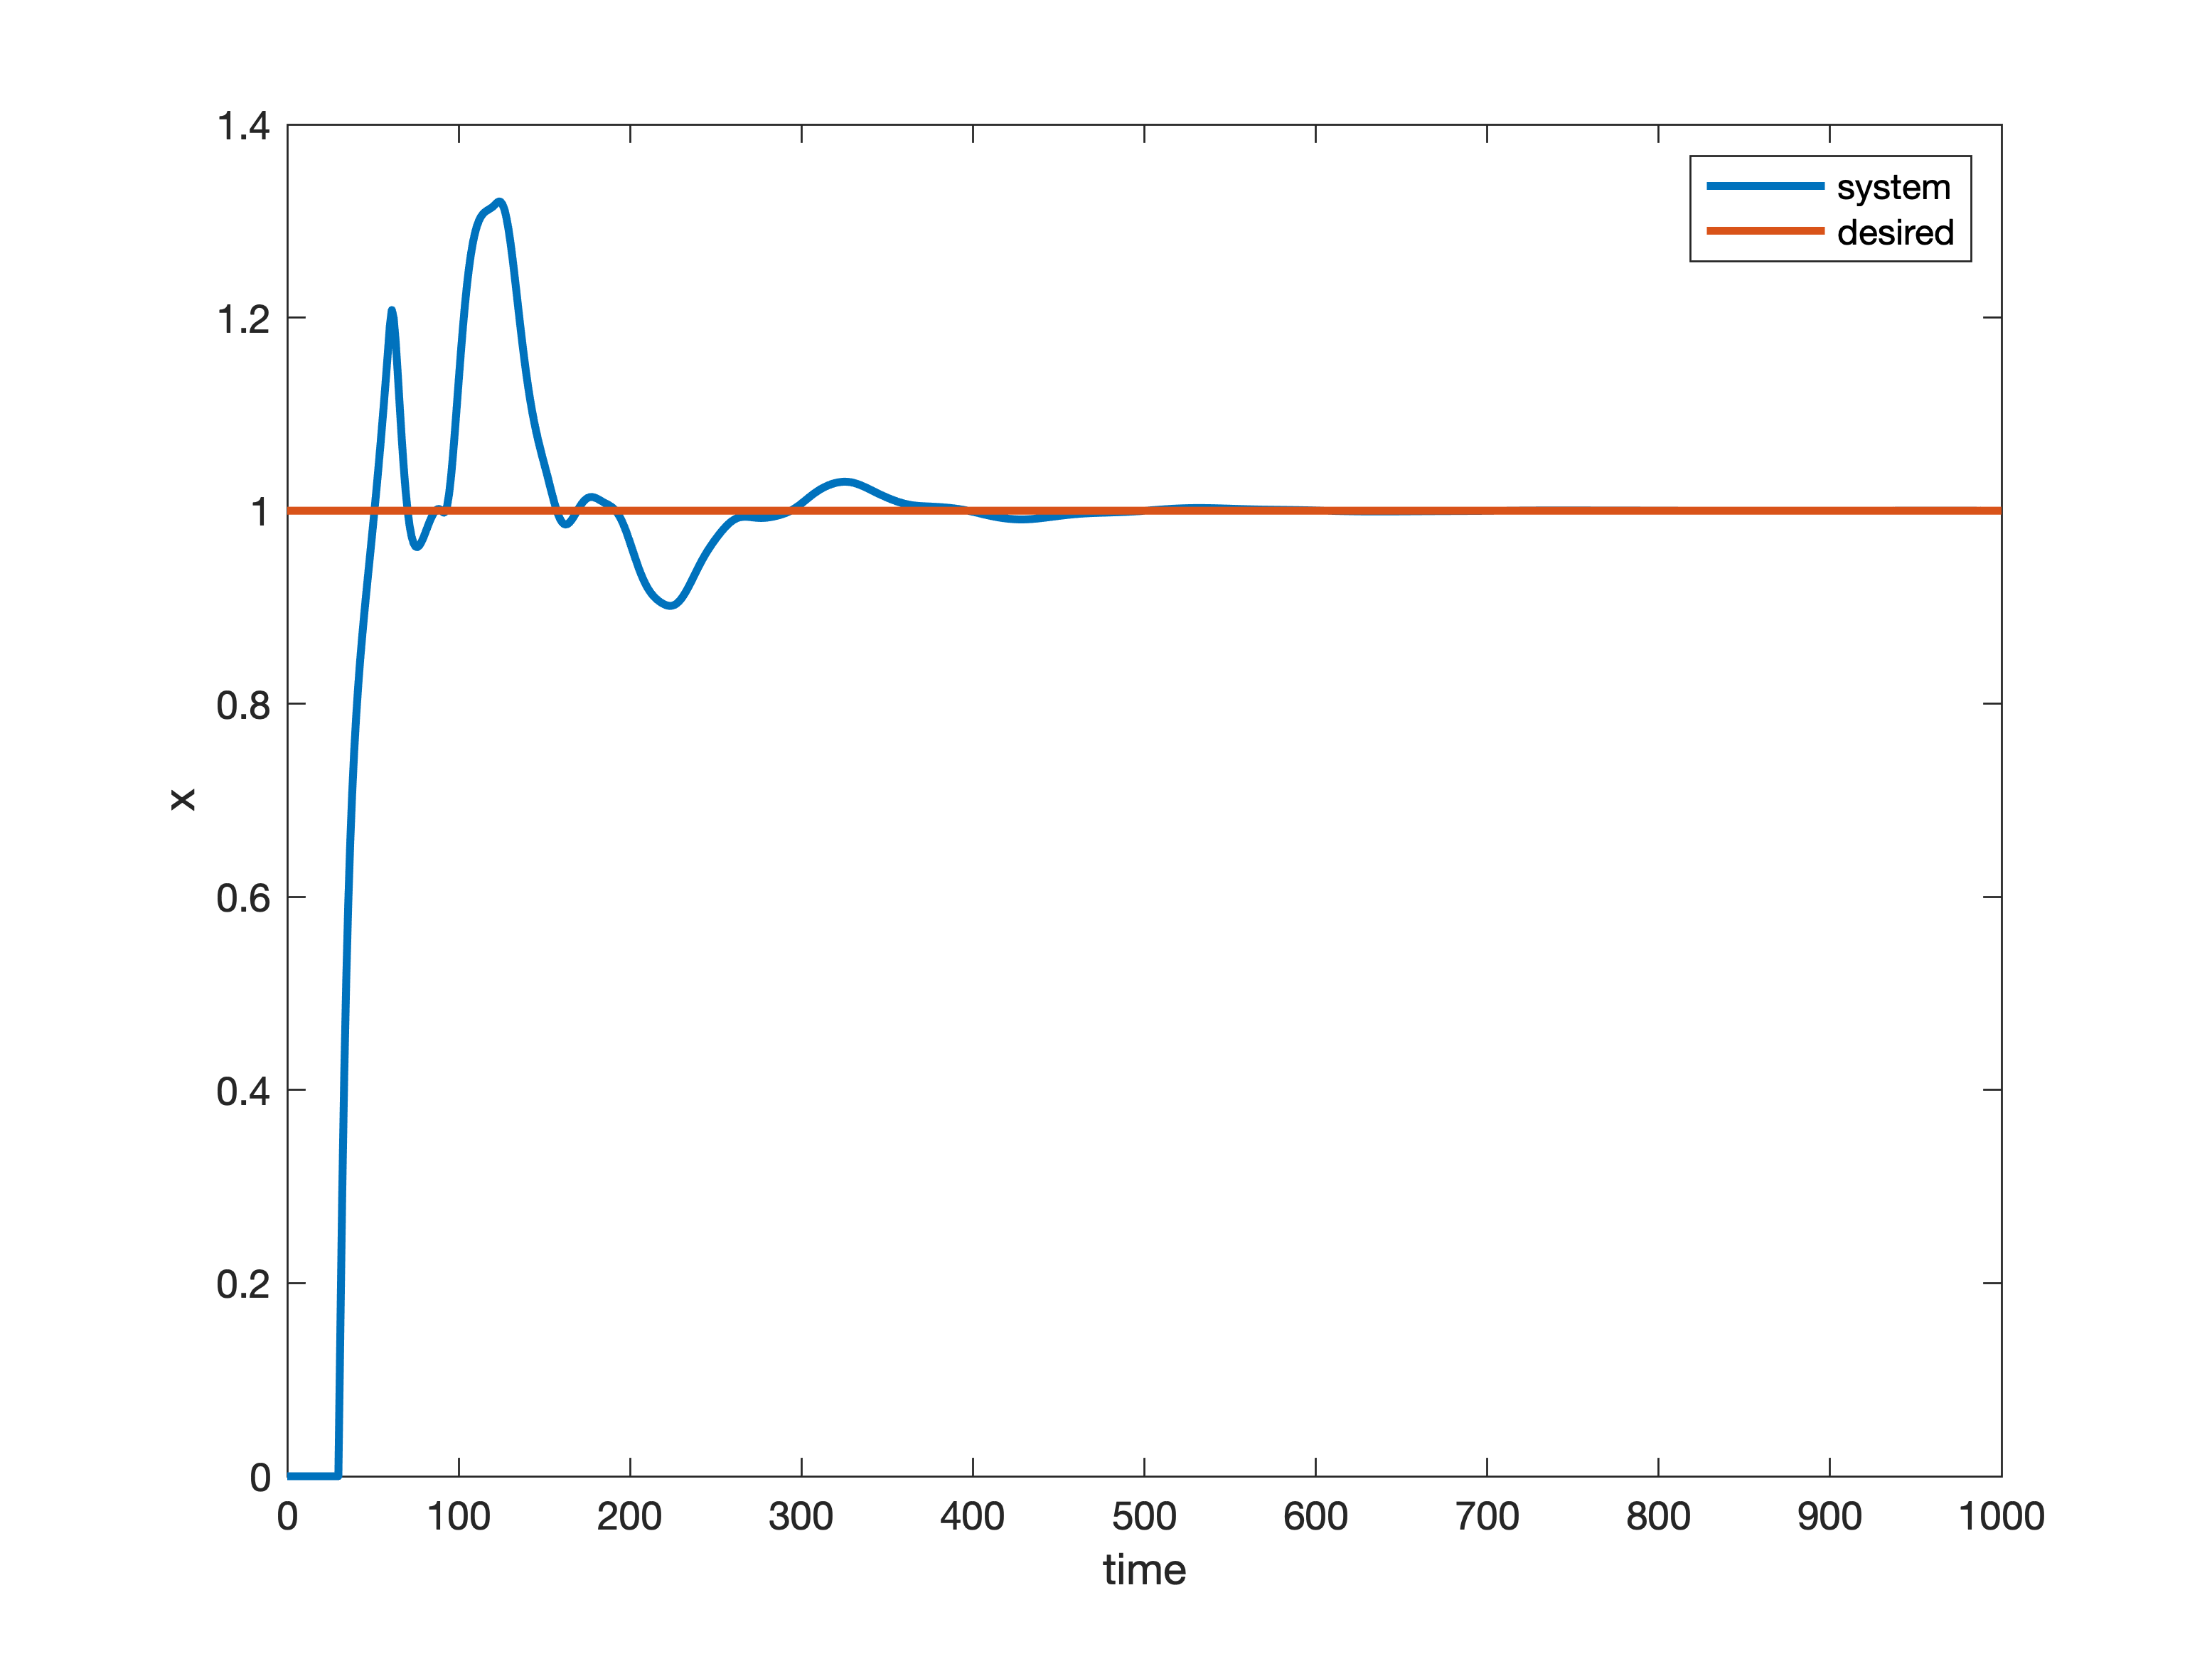
\includegraphics[width=11cm]{../Figure/Q2/IAE.png}
  \end{figure}
 \end{itemize}
 PID designed with ITAE and IAE cost function work better system is fast with lower overshoot but in ITAE cost function system has better undershoot.